\documentclass{article}
usepackage[utf8]{inputenc}

\usepackage{graphicx, subcaption}
\usepackage[spanish]{babel}
%\usepackage{indentfirst} for APA margins and French indention
\usepackage{url}
%-------------------------------------------------------------------------------
% Configuring customized document margins
%-------------------------------------------------------------------------------
\usepackage{geometry}
addtolength{\oddsidemargin}{-.75in}
addtolength{\evensidemargin}{-.75in}
addtolength{\textwidth}{1.4in}

\addtolength{\topmargin}{-0.25in}
\addtolength{\textheight}{1.65in}

%-------------------------------------------------------------------------------
% Configuring colors to make Python codes easy readable
%-------------------------------------------------------------------------------
\usepackage{listings}
\usepackage{color}

%-------------------------------------------------------------------------------
% Title region
%-------------------------------------------------------------------------------
\title{
Tarea 1: Representación de redes a través de la teoría de grafos
}
\author{Maday Hernández Quevedo}
\date{\today}

\begin{document}
\raggedright
\maketitle

\section*{Introducción}

La teoría de grafos tiene aplicaci\'n en diversas áreas, debido a que las redes aparecen prácticamente en todas las actividades de nuestra vida diaria: sistemas de comunicaciones, sistemas hidráulicos, circuitos eléctricos y electrónicos, sistemas mecánicos, redes sociales, entre otros. 

Como menciona Ravindra \cite{ahuja2017network}, las redes físicas son quizás las más comunes y mejor identificables tipos de redes. Sistemas de transporte, ya sea por carretera o rieles, suelen modelarse en sistemas de distribución complejos y decisiones logísticas.

Un ejemplo típico de investigación de operaciones es el problema de transporte. En este, un transportista con inventario de mercancías en sus almacenes debe enviar estos productos a centros minoristas geográficamente dispersos, cada uno con una demanda dada del cliente, donde el objetivo es incurrir en los mínimos gastos de transporte posibles. 

Otro ejemplo representativo de uso de grafos son los algoritmos de búsqueda web de Google, que se basan en el gráfico WWW, que contiene todas las páginas web como vértices y los  hipervínculos como bordes. \cite{chung2010graph}

La teoría de los grafos ha sido muy también ha sido usada en en química, debido a la posibilidad de representar los modelos estructurales mediante diagramas. En un grafo molecular, los vértices representan a los átomos y los lados a los enlaces químicos que conectan ciertas parejas de átomos. \cite{amador}

\section{Grafo simple no dirigido acíclico}

La mayoría de los esquemas de líneas de autobuses, tranvías o trenes del transporte público pueden ser representados por grafos simples no dirigidos acíclicos.

A continuación se muestra un sección ochos estaciones de la Línea 2 del Metro de Monterrey, donde las estaciones son los nodos y el tramo de línea entre ellos, los vértices. 

\lstinputlisting[language=Python, caption=Representación con un grafo de ocho estaciones de la Línea 2 del Metro de Monterrey.]{1.py}

\begin{figure}
  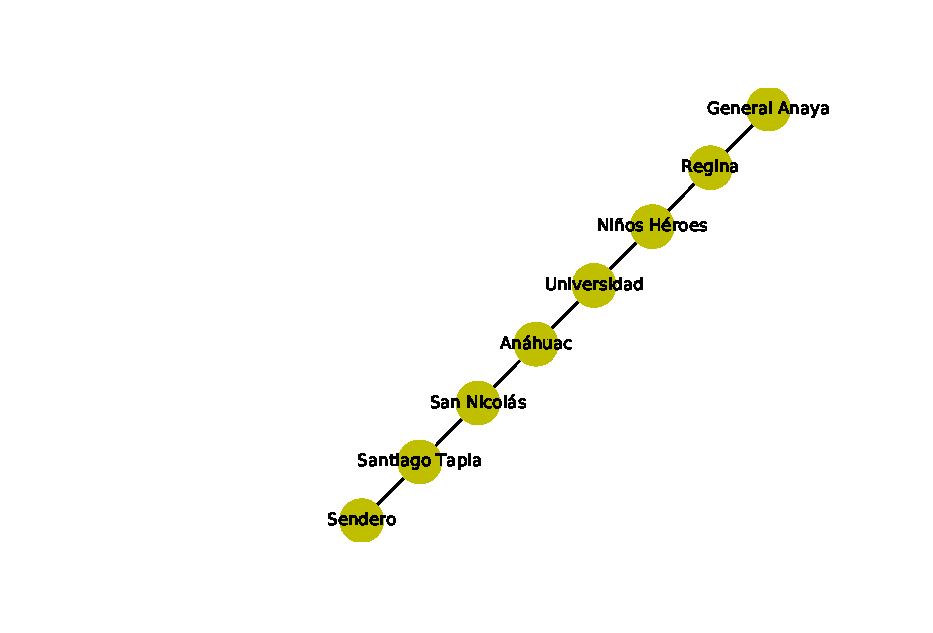
\includegraphics[width=.8\columnwidth]{1.eps}
  \caption{Representación con un grafo de ocho estaciones de la Línea 2 del Metro de Monterrey.}
  \label{fig:1}
\end{figure}

\section{Grafo simple no dirigido cíclico}

Dentro de esta categoría se pueden encontrar: relaciones comerciales entre empresas, relaciones de parentezco, amistad o romance entre personas, entre otros. 
 A continuaci\'n se muestra un grafo que representa las relaciones de amistad en un grupo de 10 personas.
 
\lstinputlisting[language=Python, caption=Relaciones de amistad en un grupo de personas.]{2.py}

\begin{figure}
  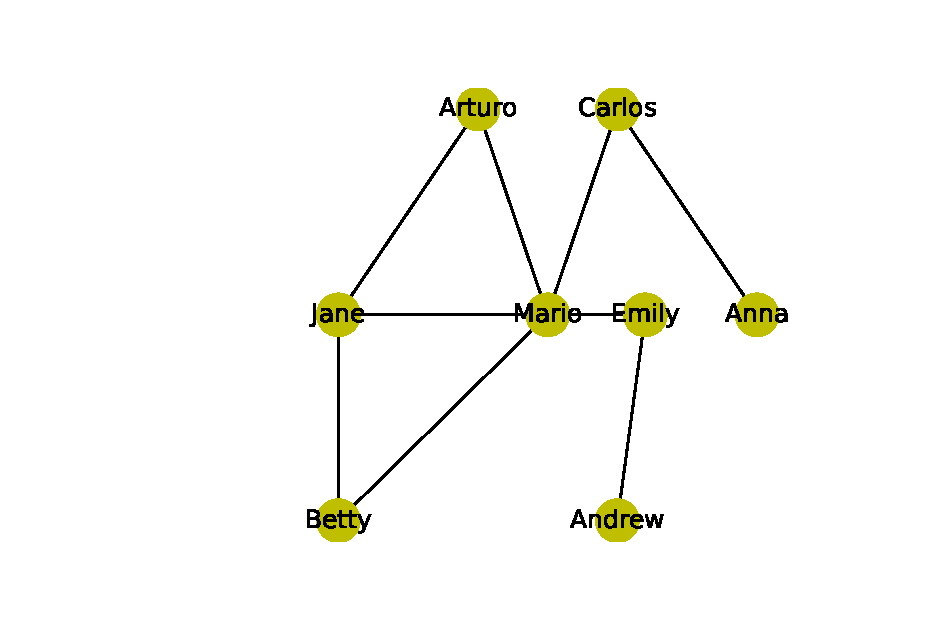
\includegraphics[width=.8\columnwidth]{2.eps}
  \caption{Relaciones de amistad en un grupo de personas.}
  \label{fig:2}
\end{figure}

\section{Grafo simple no dirigido reflexivo}



\section{Grafo simple dirigido acíclico}

La cadena de propagación de las ITS (Infecciones de Transmisión Sexual) para las cuales no se conoce cura o las que solo afectan al individuo una vez en la vida, pueden representarse mediante grafos simples dirigidos acíclicos. En este caso, el portador cada sujeto es un vértice y la dirección de transmisión de la enfermedad, es representada en la arista, desde la presona portador hacia el sujeto sano que posteriormente se convierte en portador y contagia a otros sujetos sanos.

\lstinputlisting[language=Python, caption=Representación de l la transmisión de una ITS en un grupo de personas.]{4.py}
\begin{figure}
  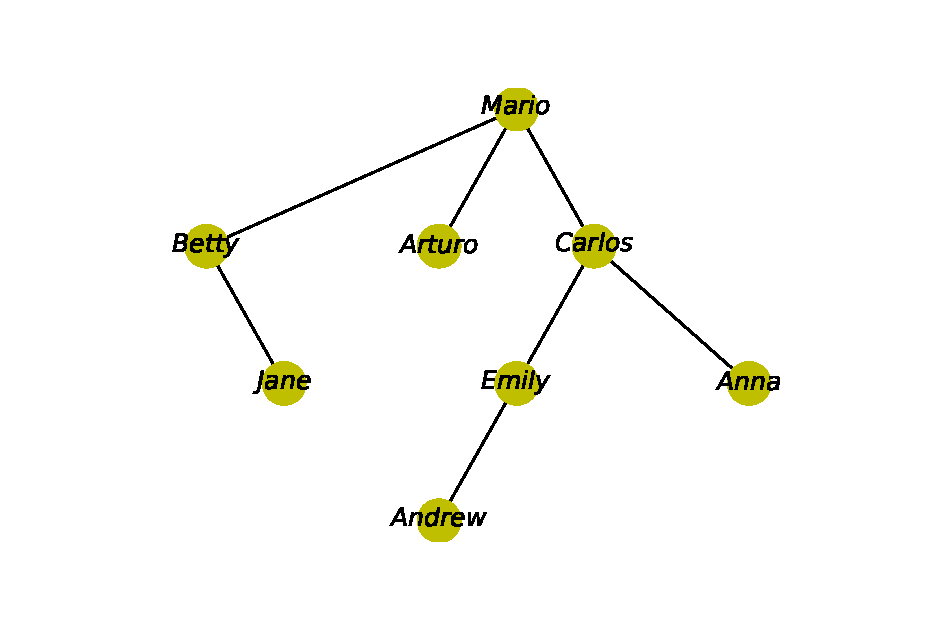
\includegraphics[width=.8\columnwidth]{4.eps}
  \caption{Representación de l la transmisión de una ITS en un grupo de personas.}
  \label{fig:4}
\end{figure}

\section{Grafo simple dirigido cíclico}

En ciudades con carreteras estrechas como Santiago de Cuba, en diferentes sectores, las carreteras son de un solo sentido y se representan con grafos de este tipo. Las aristas representan las calles y los vértices son las intersecciones entre al menos dos aristas.

\lstinputlisting[language=Python, caption= Representación de carreteras de doble sentido en Santiago de Cuba.]{5.py}
\begin{figure}
  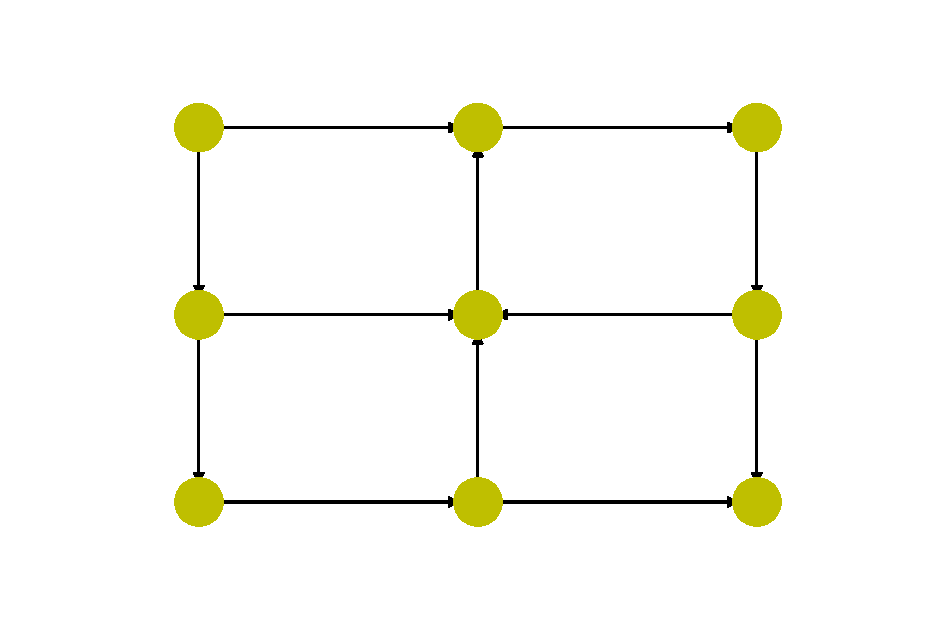
\includegraphics[width=.8\columnwidth]{5.eps}
  \caption{Carreteras de sentido único en Santiago de Cuba.}
  \label{fig:5}
\end{figure}


\section{Grafo simple dirigido reflexivo}

Un grafo en el que cada vértice es una empresa de servicios y las aristas, cada una de las otras empresas a las que le presta servicios, puede representarse mediante un grafo dirigido reflexivo pues algunas de estas empresas se brindan servicio a ellas mismas. 

Una una página web pequeña a la cual se accede a todos sus vínculos a través de un menú estático también se puede representar con este tipo de grafo. 

Otro ejemplo está dado por la representación de un grupo de personas conectadas a una red social y los perfiles de otras personas que tengan abiertos en el navegador en ese momento. Cada una de esas persona también pudiesen estar mirando su propio perfil. En la siguiente imagen puede apreciarse en color rojo que Mayra y Andrew tienen abiertos sus propios perfiles.

\lstinputlisting[language=Python, caption= Representación de carreteras de doble sentido en Santiago de Cuba.]{6.py}
\begin{figure}
  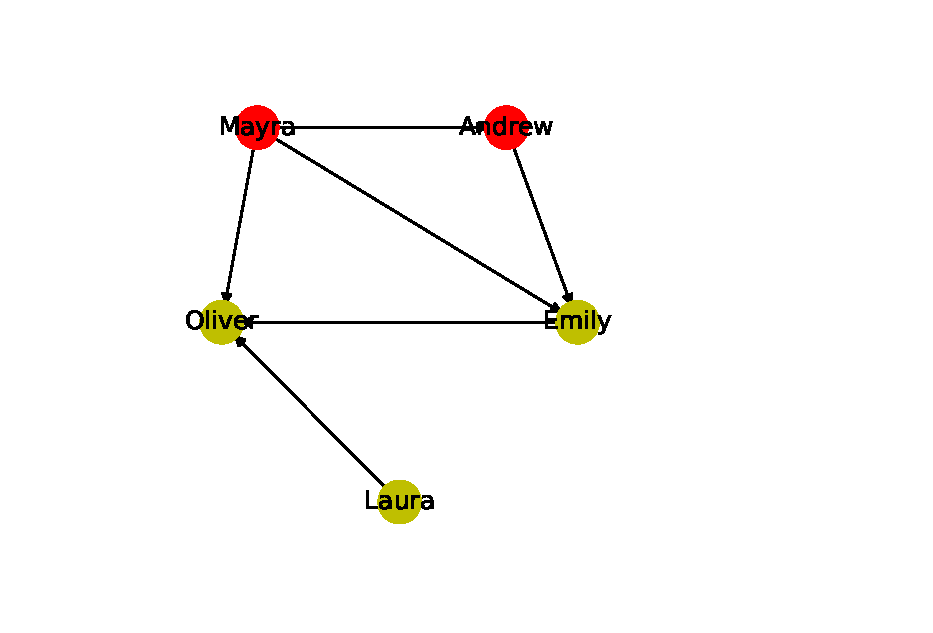
\includegraphics[width=.8\columnwidth]{6.eps}
  \caption{Red de carreteras de sentido único en Santiago de Cuba.}
  \label{fig:6}
\end{figure}




\section{Multigrafo no dirigido acíclico}

La ruta entre Santiago de Cuba y Holguín puede representarse  como un multigrafo no dirigido cíclico. En un pueblo llamado Caballería la carretera principal se bifurca, pudiendo continuar por la ruta principal hasta Banes, o por el camino alternativo de Caballería, que, aunque es más largo, puede recorrerse en menor tiempo a causa del poco tránsito.

\lstinputlisting[language=Python, caption= Representación de carreteras de doble sentido en Santiago de Cuba.]{7.py}
\begin{figure}
  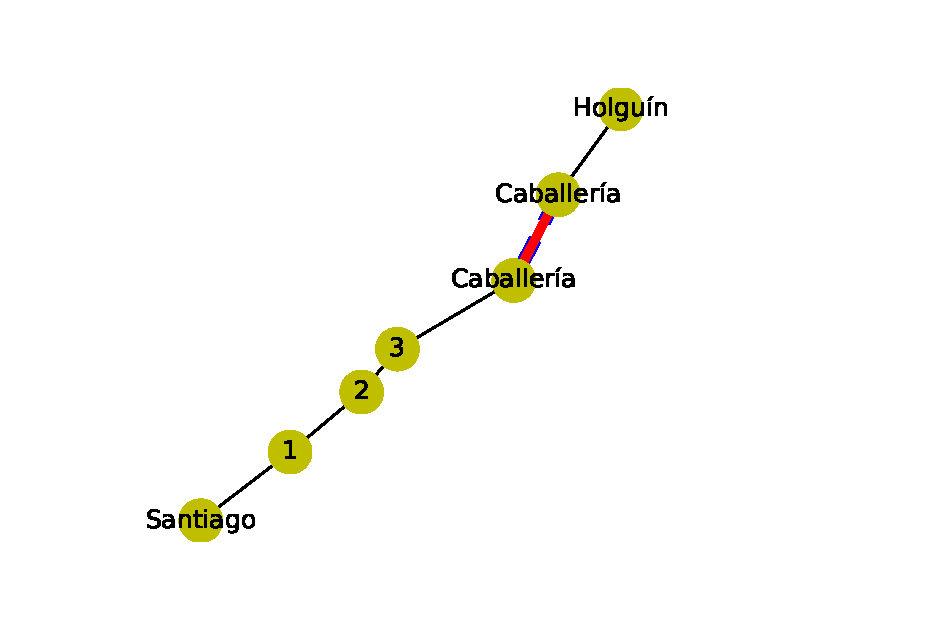
\includegraphics[width=.8\columnwidth]{7.eps}
  \caption{Red de carreteras de sentido único en Santiago de Cuba.}
  \label{fig:7}
\end{figure}

\section{Multigrafo no dirigido cíclico}

En la presa del Cacao, ubicada en el Municipio Cotorro, Ciudad de La Habana, se realizó un proyecto para favorecer la agricultura. Al rededor de la presa se construyeron una serie de canales para mantener el suelo húmedo durante todo el año. Este sistema puede ser representado mediante el grafo mostrado a continuación, el cual los vértices representan la unión entre uno o más canales y las aristas, cada uno de los canales.


\section{Multigrafo no dirigido reflexivo}


\section{Multigrafo dirigido acíclico}

Estos grafos pueden utilizarse para representar la cuenca hidrográfica de un río en su flujo hacia el mar. Los vértices representan los puntos en los que al menos dos ramificaciones del delta confluyen o se separan.

\section{multigrafo dirigido cíclico}

Cuatro amigos desean salir de vacacione

\section{multigrafo dirigido reflexivo}
González-Cervantes \cite{gonzalez2016potencial} empleó teoría de grafos para representar el potencial eléctrico en el corazón, demostrando se pueden incorporar las leyes fisiológicas involucradas. Cada uno de los vértices representa uno de los puntos principales que generan los impulsos eléctricos y que llevan la electricidad a
cada parte del corazón, las aristas describen el valor máximo de voltaje y su
duración en tiempo que descarga cada vértice. Además, puede proporcionar información con respecto al potencial eléctrico por zonas para una mejor localización.
En la imagen se muestra la representación con grafos del intervalo PR.
\lstinputlisting[language=Python, caption= Representación con grafos del intervalo PR.]{12.py}
\begin{figure}
  \centering 
  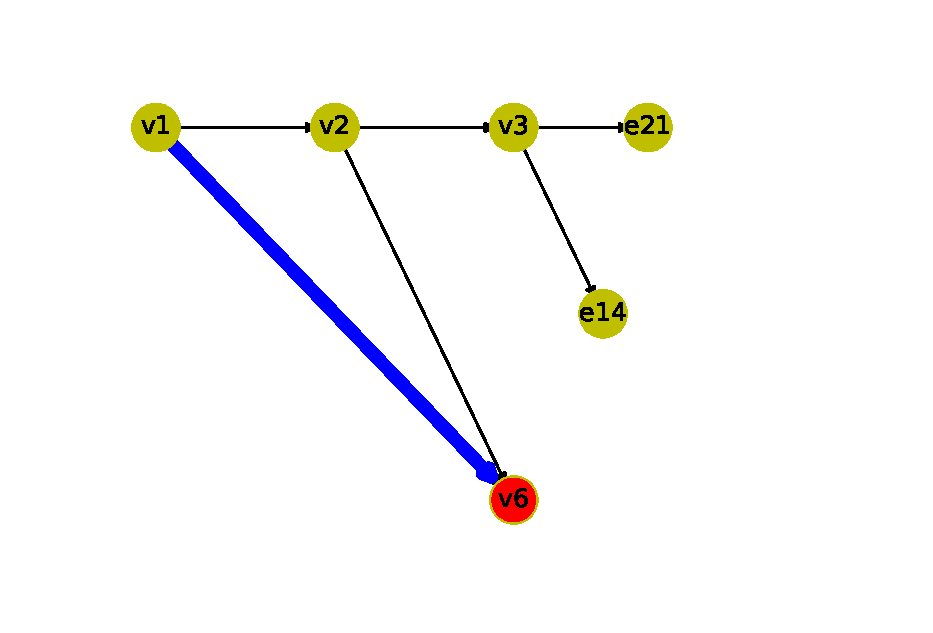
\includegraphics[width=.8\columnwidth]{12.eps}
  \caption{Representación con grafos del intervalo PR.}
  \label{fig:12}
\end{figure}


%-------------------------------------------------------------------------------
% References
%-------------------------------------------------------------------------------
\newpage
\bibliography{1}
\bibliographystyle{plain}



\end{document}